\documentclass[12pt]{article}

\usepackage{sbc-template}
\usepackage[hidelinks]{hyperref}
\usepackage{graphicx,url}
\usepackage{xcolor}
\usepackage{float}

\usepackage[brazil]{babel}   
%\usepackage[latin1]{inputenc}  
\usepackage[utf8]{inputenc}
     
\sloppy

\title{\textbf{Arduino Sensor Kit da Yahboom Technology:\\Tutorial para Experimentos}}

\author{Raul Ramires\inst{1}}


\address{Departamento de Informática -- Universidade Estadual de Maringá
	(UEM)\\
	Maringá -- PR -- Brazil
	\email{ra82293@uem.br}
}

\begin{document} 

\maketitle

\section{Introdução}
	O arduino é uma placa microcontroladora baseada no microcontrolador ATMega e pode ser integrada com uma grande diversidade de componentes e sensores. O projeto a ser desenvolvido propõe a configuração do ambiente de trabalho e a realização de diversos experimentos com diferentes sensores.

	O Arduino Sensor Kit da da Yahboom Technology, utilizado é um kit de componentes e sensores baseado no Arduino UNO R3. O objetivo do presente tutorial é o de apresentar os passos e explicações de como realizar experimentos com o referido kit. 

\section{Ambiente de Trabalho}
	O arduino possui uma IDE \textit{Integrated Development Environment} chamada de ``Arduino IDE'', que é onde serão escritos os códigos para que depois sejam enviados ao arduino e executado.

\subsection{Download da IDE}
	Para fazer o download da IDE basta ir ao \textcolor{blue}{https://www.arduino.cc/en/Main/Software} e escolher a versão de acordo com o sistema operacional utilizado, estando disponível para Windows, Linux e MacOS.

	A Figura \ref{figIDE} mostra a tela principal da IDE do arduino.

	\begin{figure}[H]
		\centering
		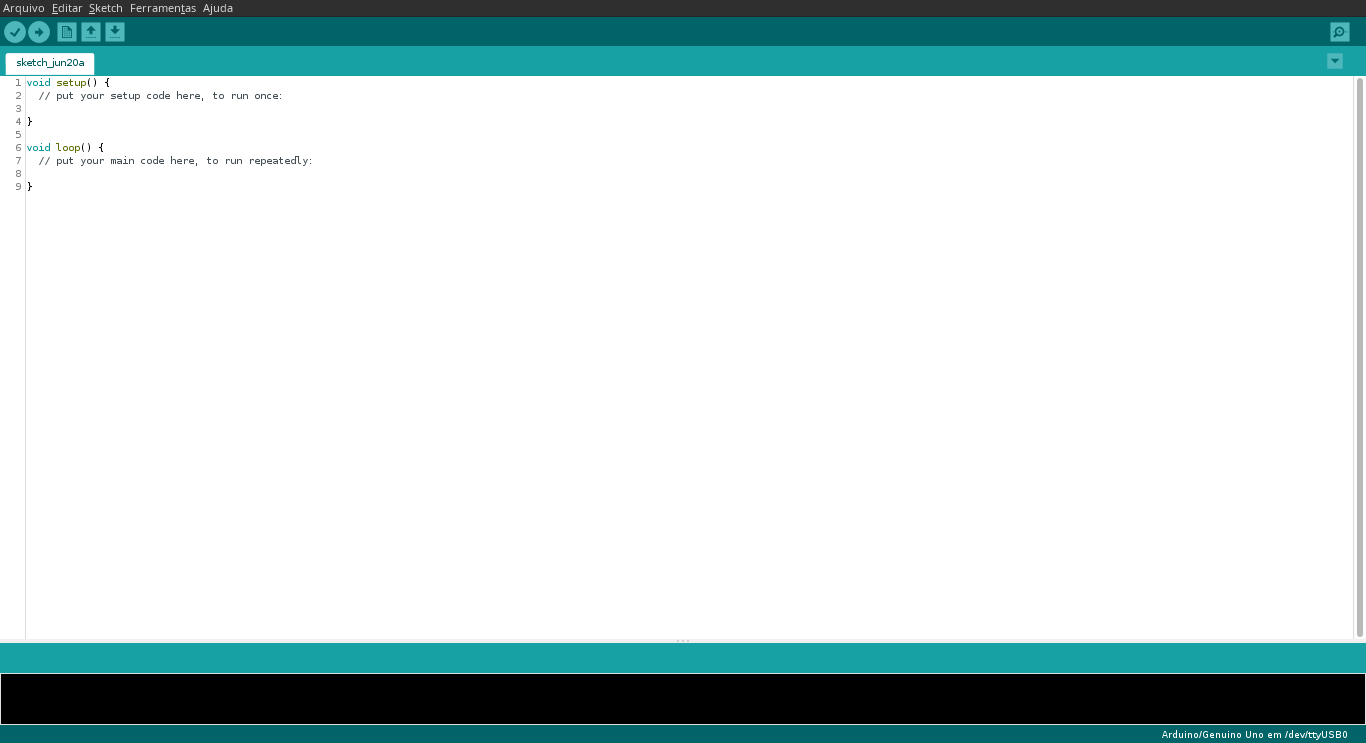
\includegraphics[scale=0.2]{Imagens/telaIDE.png}
		\caption{Tela principal da Arduino IDE.}
		\label{figIDE}
	\end{figure}

\subsection{Arduino Sensor Kit}
	O kit de sensores para arduino UNO da Yahboom contém os seguintes componentes:

\begin{description}
	\item[Protoboard] Placa de prototipação de 830 pontos;
	\item[Arduino UNO] Microcontrolador Arduino UNO R3;
	\item[Bateria 9V] Bateria para alimentação do arduino;
	\item[Motor de Passo] Motor de passo alimentado por 5V;
	\item[Motor DC] Motor de corrente contínua;
	\item[Servo Motor] Micro Servo 9g;
	\item[Matriz de LED] Matriz 8x8 de LEDs (1588BS);
	\item[Display 7 Segmentos] Módulo com um display de 7 segmentos (5161AS);
	\item[4 Displays de 7 Segmentos] Módulo com 4 displays de 7 segmentos (3461AS-1);     
	\item[Hélice] Hélice de plástico com 4 pás;
	\item[LDR] Resistor dependente de luz;
	\item[Push Button] Botões de pressionamento;
	\item[Sensor de Presença] Sensor infravermelho de presença;
	\item[Sensor de Gás] Sensor de gás \textit{Flying-Fish};
	\item[Sensor Gray Scale] Sensor de escala de cinza;
	\item[Sensor Touch] Sensor de toque capacitivo; 
	\item[Joystick] Módulo joystick de 3 eixos;
	\item[Sensor de Som] Módulo de sensor de som;
	\item[LED Flashlight] Módulo composto por 2 LEDs RGB;
	\item[Sensor Ultrasônico] Sensor ultrasônico de distância (HC-SR04);
	\item[Display LCD] Display LCD 16x2;
	\item[Potenciômetro] Resistor varável de 5k$\Omega$;
	\item[Ponte H] Módulo para controle de motores;
	\item[LEDs] 15 LEDs coloridos;
	\item[Resistores] Resistores de 220$\Omega$, 1k$\Omega$ e 10k$\Omega$;
	\item[Buzzer] Buzzer ativo para emitir som.      
\end{description}

	A Figura \ref{figComponentes} mostra os componentes descritos acima.

	\begin{figure}[H]
		\centering
		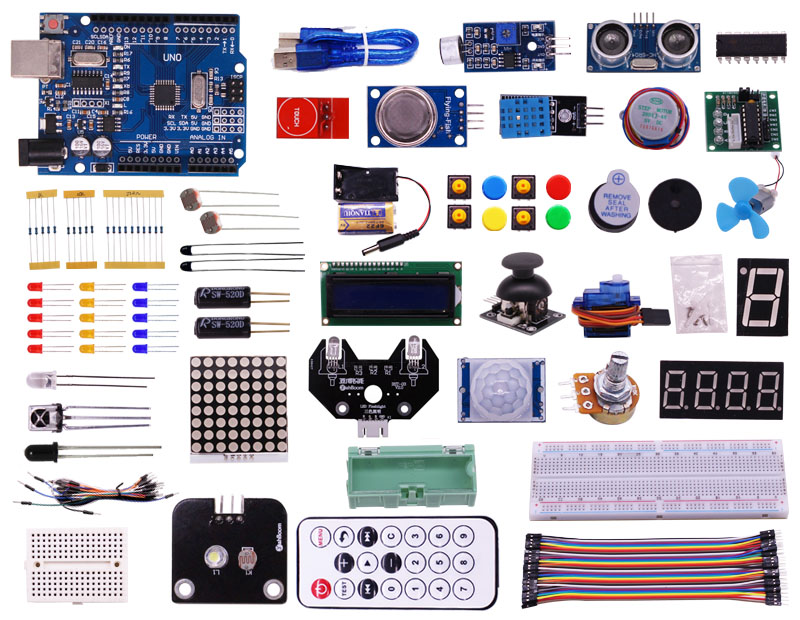
\includegraphics[scale=0.25]{Imagens/kit.png}
		\caption{Sensores presentes no kit.}
		\label{figComponentes}
	\end{figure}

\section{Programação}
	A programação do arduino é feita na linguagem C++ e possui uma grande quantidade de bibliotecas prontas para a utilização de sensores.

\subsection{Estrutura do código}
	A Figura \ref{figEstruturaCodigo} mostra a estrutura básica de um código para arduino. Esse código é dividido em duas funções: a função \textit{setup} e a função \textit{loop}.

	\begin{figure}[H]
		\centering
		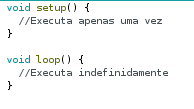
\includegraphics[scale=1]{Imagens/figEstrutura.png}
		\caption{Estrutura do código.}
		\label{figEstruturaCodigo}
	\end{figure}

	A função \textit{setup} será executada apenas uma vez no início do programa, geralmente é aqui que ficam as definições de pinos de entradas e saídas e algumas variáveis globais.
	A função \textit{loop} será executada infinitamente enquanto o arduino estiver ligado, é aqui que serão feitas as leituras de sensores e decisões de ações com bases nos dados lidos dos sensores.

\subsection{Upload do código}
	Para realizar o \textit{upload} do código para a placa do arduino, basta clicar no botão ``carregar'', então o código será compilado e carregado para o arduino e então começar a execução.

	A Figura \ref{figCarregarIDE} mostra em destaque o botão para carregar o código para o arduino.

	\begin{figure}[H]
		\centering
		
\includegraphics[scale=1]{Imagens/carregarIDE.png}
		\caption{Destaque do botão de carregar.}
		\label{figCarregarIDE}
	\end{figure}

\section{Experimentos}
	Nessa seção serão realizados vários experimentos com o arduino, utilizando uma grande diversidade de componentes e sensores.

	Todos os experimentos realizados nesse trabalho estão disponíveis no repositório no \href{https://github.com/ramires352/Arduino-UEM}{\underline{\textcolor{blue}{\textit{GitHub}}}} e os esquemáticos dos circuitos estão disponíveis no \href{https://www.tinkercad.com/users/8OFhdueEmAr-rrramires?category=circuits&sort=likes&view_mode=default}{\underline{\textcolor{blue}{\textit{Tinkercad}}}}.

\subsection{Piscar um LED}
	Para realizar esse experimentos será necessário um LED, uma \textit{protoboard} e dois \textit{jumpers}.

	A \textit{protoboard} é construída como uma matriz, onde cada coluna possui 5 pontos de contato que são interligados entre si, porém uma coluna é isolada de sua vizinha, sendo necessário a utilização de um \textit{jumper} para interligar duas colunas.

	Alguns modelos de \textit{protoboard} possuem dois barramentos laterais, um negativo e um positivo que percorrem a \textit{protoboard} inteira. O padrão de utilização desses barramentos é ligar o 5V no barramento vermelho e o GND no barramento preto, ficando assim mais simples de realizar a alimentação dos componentes utilizados.

	A Figura \ref{figProtoboard} mostra o esquema de uma \textit{protoboard} de 360 pontos.

	\begin{figure}[H]
		\centering
		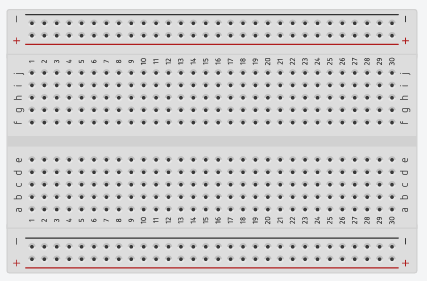
\includegraphics[scale=0.5]{Imagens/figProtoboard.png}
		\caption{\textit{Protoboard} de 360 pontos}
		\label{figProtoboard}
	\end{figure}

	A Figura \ref{figExp1PiscarLEDesq} mostra o esquema do circuito para piscar um LED, utilizando o arduino.

	\begin{figure}[H]
		\centering
		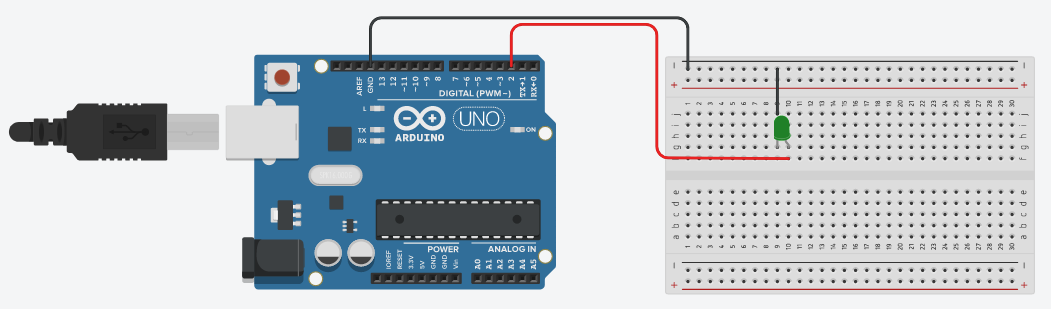
\includegraphics[scale=0.3]{Imagens/Experimentos/1-PiscarLED/1-PiscarLED.png}
		\caption{Esquemático do circuito do experimento 1.}
		\label{figExp1PiscarLEDesq}
	\end{figure}

	Nesse circuito o pino digital 2 do arduino está ligado na coluna 10 da protoboard, onde, nessa mesma coluna está ligado o terminal positivo do LED. O terminal negativo do LED está ligado na coluna 9, que possui um \textit{jumper} para o barramento preto, que por sua vez está ligado ao GND do arduino. Sendo assim o LED irá acender quando o arduino enviar o sinal de 5V no pino 2.

	A Figura \ref{figExp1PiscarLEDcod} mostra o código que fará com que o arduino pisque o LED.

	\begin{figure}[H]
		\centering
		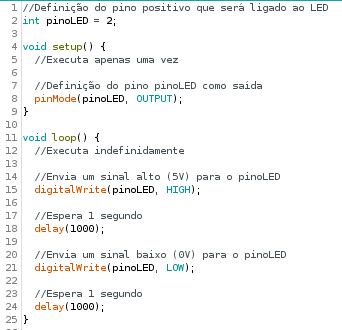
\includegraphics[scale=0.7]{Imagens/Experimentos/1-PiscarLED/1-PiscarLEDcod.png}
		\caption{Código do experimento 1.}
		\label{figExp1PiscarLEDcod}
	\end{figure}

\subsection{Mudar o brilho de um LED}
	Para realizar esse experimento será necessário um LED, um potenciômetro e um resistor de 220$\Omega$.

	O potenciômetro é um resistor capaz de variar sua resistencia, para esse experimento, o arduino irá ler esse valor de resistência e associar a um valor de tensão e enviar ao LED, variando assim o brilho do LED. Como esse valor é variável, é necessário conectar o potenciômetro a uma porta analógica do arduino.

	A Figura \ref{figExp2BrilhoLEDesq} mostra o esquemático do circuito do experimento.

	\begin{figure}[H]
		\centering
		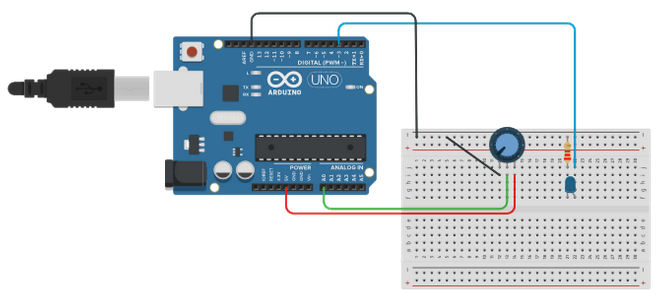
\includegraphics[scale=0.4]{Imagens/Experimentos/2-brilhoLED/2-brilhoLEDesq.png}
		\caption{Esquemático do circuito do experimento 2.}
		\label{figExp2BrilhoLEDesq}
	\end{figure}

	O arduino faz a leitura do potenciômetro em um valor de 0 a 1023. Para usar esse valor para acender o LED, é necessário fazer uma conversão para um valor de 0 a 255. Para isso é utilizado a função \textit{map}, que é responsável por fazer esse mapeamento de um intervalo para outro.

	A figura \ref{figExp2BrilhoLEDcod} mostra o código do experimento 2.

	\begin{figure}[H]
		\centering
		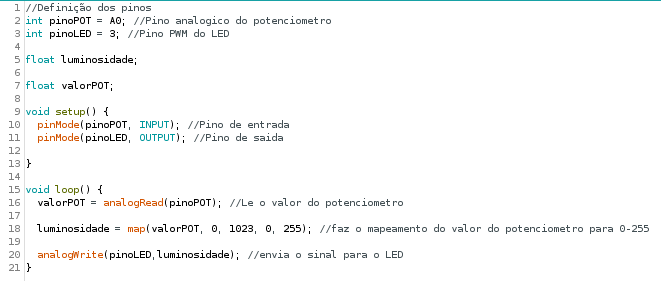
\includegraphics[scale=0.6]{Imagens/Experimentos/2-brilhoLED/2-brilhoLEDcod.png}
		\caption{Código do experimento 2.}
		\label{figExp2BrilhoLEDcod}
	\end{figure}

\subsection{Sensor de luz}
	Esse experimento tem como objetivo controlar uma barra de LEDs a partir de um LDR (\textit{Light Dependent Resistor}). O LDR é um resistor que varia sua resistência de acordo com a luz que incide sobre ele, quanto maior a quantidade de luz, menor a resistência do LDR. Como o LDR é um componente que possui um valor de resistência variável, é necessário conectá-lo a uma porta analógica do arduino.

	Para esse experimento, quanto maior a luz incidente sobre o LDR, menos LEDs irão acender.

	A Figura \ref{figExp3LDResq} mostra o esquemático do circuito do experimento 3.

	\begin{figure}[H]
		\centering
		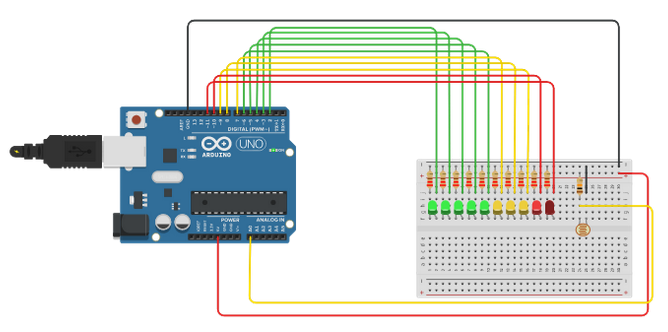
\includegraphics[scale=0.4]{Imagens/Experimentos/3-LDR-LEDGraph/3-LDR-LEDGraphEsq.png}
		\caption{Esquemático do circuito do experimento 3.}
		\label{figExp3LDResq}
	\end{figure}

	A Figura \ref{codigoExp3} mostra o código do experimento 3.

	\begin{figure}[H]
		\centering
		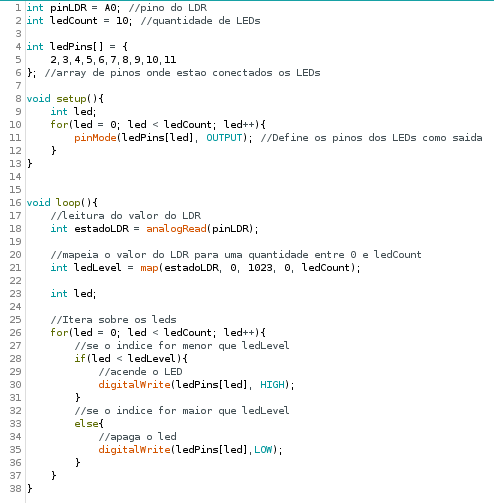
\includegraphics[scale=0.39]{Imagens/Experimentos/3-LDR-LEDGraph/codigo.png}
		\caption{Código do experimento 3.}
		\label{codigoExp3}
	\end{figure}

\subsection{Display de 7 Segmentos}
	Esse experimento faz o controle de um display de 7 segmentos utilizando um botão para exibir os dígitos de 0 a 9. O display incia exibindo o dígito 0 e incrementa um dígito quando o botão é pressionado. Os segmentos do display são nomeados de acordo com a Figura \ref{figSegmentosDisplay} \cite{siteDisplay7}.

	\begin{figure}[H]
		\centering
		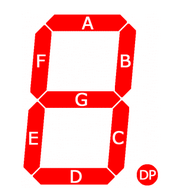
\includegraphics[scale=0.5]{Imagens/Experimentos/4-Display7Seg/7segmentos.png}
		\caption{Segmentos do display.}
		\label{figSegmentosDisplay}
	\end{figure}

	Para acender um segmento o arduino deve enviar um sinal alto para o segmento, e para apagar deve enviar um sinal baixo.

	A Figura \ref{figPinosDisplay} mostra a pinagem do display. Para esse experimento não será utilizado o ponto decimal.

	\begin{figure}[H]
		\centering
		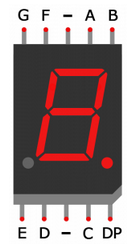
\includegraphics[scale=0.5]{Imagens/Experimentos/4-Display7Seg/pinosDisplay.png}
		\caption{Pinagem do display de 7 segmentos.}
		\label{figPinosDisplay}
	\end{figure}

	O botão é definido como \textit{INPUT\_PULLUP} para utilizar um resistor interno do arduino e simplificar o circuito, por conta disso, o arduino interpreta o botão como estado alto quando não pressionado e estado baixo quando pressionado. Para detectar o acionamento do botão é necessário considerar o estado atual do botão e o estado anterior, pois o arduino faz a leitura do botão um grande número de vezes por segundo, sendo assim é necessário esse tratamento para evitar que o arduino interprete que o botão foi acionado diversas vezes em apenas um acionamento.

	A Figura \ref{figExp4cod} mostra o esquemático do circuito do experimento 4.

	\begin{figure}[H]
		\centering
		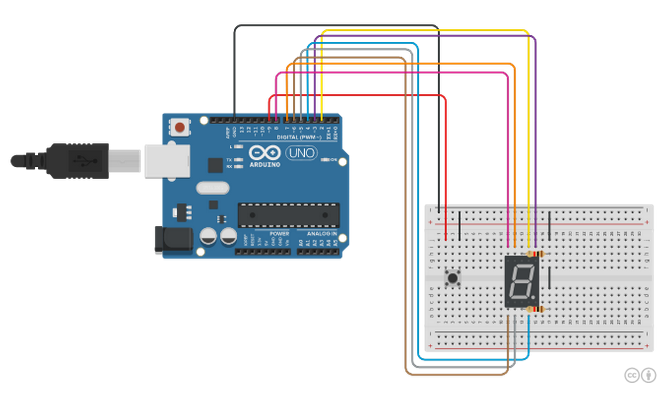
\includegraphics[scale=0.3]{Imagens/Experimentos/4-Display7Seg/esquematico.png}
		\caption{Esquemático do experimento 4.}
		\label{figExp4cod}
	\end{figure}

	A Figura \ref{figExp4botao} mostra o trecho de código que faz a leitura do botão.

	\begin{figure}[H]
		\centering
		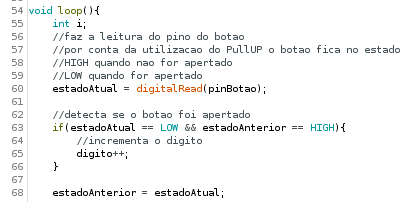
\includegraphics[scale=0.65]{Imagens/Experimentos/4-Display7Seg/codigoBotao.png}
		\caption{Código que detecta o acionamento do botão.}
		\label{figExp4botao}
	\end{figure}

\subsection{Matriz de LEDs 8x8}
Esse experimento tem como objetivo percorrer os LEDs da matriz utilizando um joystick.

Como o \textit{Tinkercad} não possui os módulos da matriz e do joystick, esse experimento não estará disponível para simulação.

A Figura \ref{figPinosMatriz} mostra a numeração de pinos da matriz de LEDs \cite{siteLEDMatrix}.

\begin{figure}[H]
	\centering
	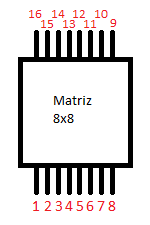
\includegraphics[scale=0.7]{Imagens/Experimentos/5-LEDMatrix/pinosMatriz.png}
	\caption{Numeração de pinos da matriz.}
	\label{figPinosMatriz}
\end{figure}

A Tabela \ref{tabMatrizLinhas} mostra como fazer a conexão das linhas da matriz com o arduino.

\begin{table}[H]
	\centering
	\begin{tabular}{|c|c|c|}
	\hline
	\textbf{Linha} & \textbf{Pino Matriz} & \textbf{Pino Arduino} \\ \hline
	1              & 9                    & 2                     \\ \hline
	2              & 14                   & 3                     \\ \hline
	3              & 8                    & 4                     \\ \hline
	4              & 12                   & 5                     \\ \hline
	5              & 1                    & 6                     \\ \hline
	6              & 7                    & 7                     \\ \hline
	7              & 2                    & 8                     \\ \hline
	8              & 5                    & 9                     \\ \hline
	\end{tabular}
	\caption{Conexão das linhas da matriz no arduino.}
	\label{tabMatrizLinhas}
\end{table}

A Tabela \ref{tabMatrizColunas} mostra como fazer a conexão das colunas da matriz com o arduino.

\begin{table}[H]
	\centering
	\begin{tabular}{|c|c|c|}
	\hline
	\textbf{Coluna} & \textbf{Pino Matriz} & \textbf{Pino Arduino} \\ \hline
	1               & 13                   & 10                    \\ \hline
	2               & 3                    & 11                    \\ \hline
	3               & 4                    & 12                    \\ \hline
	4               & 10                   & 13                    \\ \hline
	5               & 6                    & A0                    \\ \hline
	6               & 11                   & A1                    \\ \hline
	7               & 15                   & A2                    \\ \hline
	8               & 16                   & A3                    \\ \hline
	\end{tabular}
	\caption{Conexão das colunas da matriz no arduino.}
	\label{tabMatrizColunas}
\end{table}

A Figura \ref{figPinosJoystick} mostra a numeração de pinos do módulo joystick.

\begin{figure}[H]
	\centering
	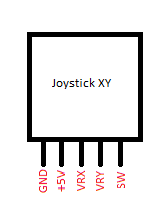
\includegraphics[scale=0.7]{Imagens/Experimentos/5-LEDMatrix/pinosJoy.png}
	\caption{Numeração de pinos do joystick.}
	\label{figPinosJoystick}
\end{figure}

Para ligar o joystick ao arduino basta ligar o \textit{GND} do módulo ao \textit{GND} do arduino, o +5V do módulo ao +5V do arduino. Os pinos VRX e VRY são ligados aos pinos A4 e A5, respectivamente.

\subsection{Sensor de Distância}
Esse experimento consiste em utilizar o sensor ultrasônico de distância para exibir a distância medida no display LCD. Esse experimento possui uma medida de distância mínima que pode ser regulada utilizando um potenciômetro. Quando a distância medida for menor que a distância mínima será soado um alarme sonoro.

O circuito possui ainda um segundo potenciômetro necessário para a regulagem do brilho do display.

Para esse experimento será necessário a utilização de duas bibliotecas, a \textbf{LiquidCrystal.h} que é responsável por controlar o display e a biblioteca \textbf{Ultrasonic.h} que controla o sensor ultrasônico de distância.

A biblioteca \textbf{LiquidCrystal.h} já está contida na IDE do arduino. Já a biblioteca \textbf{Ultrasonic.h} deve ser baixada e instalada manualmente.

Originalmente a biblioteca \textbf{Ultrasonic.h} foi desenvolvida pelo site \href{https://www.filipeflop.com/blog/sensor-ultrassonico-hc-sr04-ao-arduino/}{\textcolor{blue}{\textbf{FilipeFlop}}} \cite{siteUltrasonic}. A biblioteca está disponível no repositório do \textit{GitHub} para fácil acesso.

Para adicionar a biblioteca ao Arduino IDE basta clicar em \textit{Sketch $\rightarrow$ Incluir Biblioteca $\rightarrow$ Adicionar Biblioteca .ZIP} e selecionar o arquivo \textit{Ultrasonic.zip} presente na pasta Bibliotecas.

Como não é possível instalar bibliotecas adicionais no \textit{Tinkercad}, esse experimento não está disponível para simulação, porém é possível ver o esquemático do circuito no site, como mostrado na Figura \ref{figExp6esq}.

\begin{figure}[H]
	\centering
	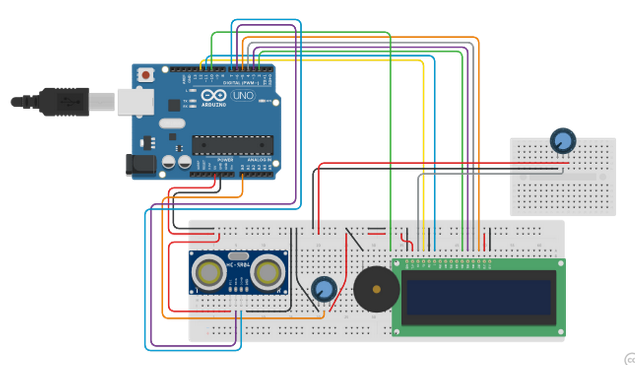
\includegraphics[scale=0.6]{Imagens/Experimentos/6-SensorDistancia/esquematico.png}
	\caption{Esquemático do experimento 6.}
	\label{figExp6esq}
\end{figure}

\subsection{LED RGB}
O objetivo desse experimento é mostrar o funcionamento de um LED RGB. O LED RGB é composto de 3 LEDs, um vermelho, um verde e um azul. A combinação dessas 3 cores geram novas cores.

O LED RGB disponível no \textit{Tinkercad} tem os pinos diferentes do módulo RGB disponível no kit utilizado para esse tutorial, porém o funcionamento é o mesmo. O LED RGB consiste em 4 terminais, um para cada cor e um pino GND.

Nesse experimento foram utilizados 3 botões para alterar cada uma das 3 cores. Foi definido um número de 3 tonalidades para cada cor, mas isso pode ser alterado no código do experimento, podendo usar até um máximo de 255 tonalidades.

O esquemático desse experimento pode ser visto na Figura \ref{figExp7esq}.

\begin{figure}[H]
	\centering
	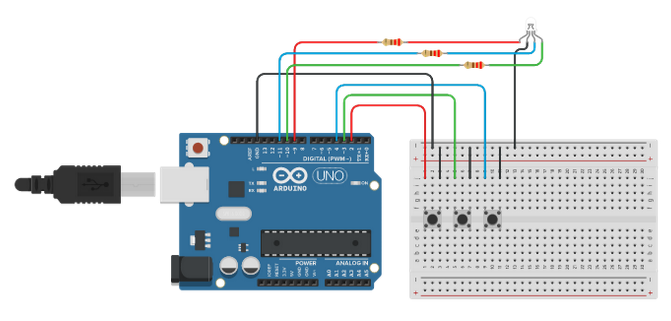
\includegraphics[scale=0.6]{Imagens/Experimentos/7-LED-RGB/esq.png}
	\caption{Esquemático do experimento 7.}
	\label{figExp7esq}
\end{figure}

\subsection{Sensor de Presença}
O objetivo desse experimento é mostrar o funcionamento de um sensor de presença. O arduino irá piscar um LED RGB quando o sensor for ativado por um movimento. O sensor possui duas regulagens, sendo uma de sensibilidade que determina o alcance do sensor, e uma de duração, que determina quanto tempo o sensor fica ativado após detectar um movimento. Ambas as regulagens são feitas por pequenos potenciômetros soldados na PCB do sensor.

O esquemático do circuito deste experimento pode ser visto na Figura \ref{figExp8esq}

\begin{figure}[H]
	\centering
	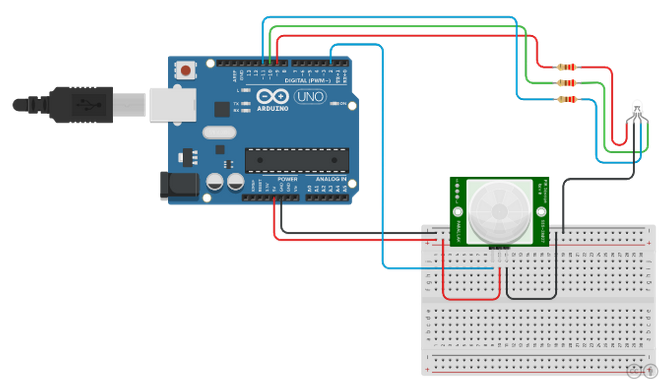
\includegraphics[scale=0.5]{Imagens/Experimentos/8-SensorPresenca/esq.png}
	\caption{Esquemático do circuito do experimento 8.}
	\label{figExp8esq}
\end{figure}

\subsection{Controle Remoto}
O objetivo desse experimento é mostrar o funcionamento de um controle remoto infra-vermelho. Para realizar a comunicação é necessário utilizar o receptor infra-vermelho, que irá receber o comando do controle remoto e converter para um valor hexadecimal, cada botão possui um valor diferente.

Para utilizar o sensor de infravermelho, é necessário instalar uma biblioteca do Arduino. Para isso adicione a biblioteca \textbf{IRremote.zip} localizada na pasta \textbf{Bibliotecas} do repositório utilizado nesse trabalho. A instalação da biblioteca é feita da mesma forma da biblioteca que foi instalada no experimento do sensor de distância.

Nesse experimento o controle remoto será utilizado para controlar a quantidade de LEDs que serão acesos. Utilizando os botoes de 0 a 5 do controle é possível determinar essa quantidade.

O esquemático do circuito pode ser visto na Figura \ref{figExp9esq}.

\begin{figure}[H]
	\centering
	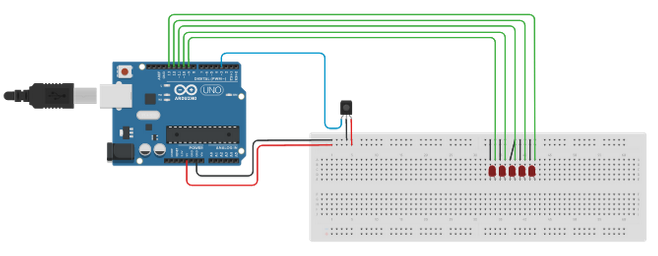
\includegraphics[scale=0.6]{Imagens/Experimentos/9-ControleRemoto/esq.png}
	\caption{Esquemático do circuito do experimento 9.}
	\label{figExp9esq}
\end{figure}

\subsection{Sensor de Som}
O objetivo desse experimento é acender ou apagar um LED utilizando um sensor de som. Esse sensor funciona apenas com a detecção de som, ou seja, quando um som for detectado o valor de saída do sensor será \textbf{LOW} e quando não for detectado um som o valor de saída será \textbf{HIGH}. O sensor possui um ajuste de sensibilidade que pode ser ajustado através de um potenciômetro soldado direto na PCB do sensor. Para esse experimento será utilizado o som de uma palma para acionar o LED, então a sensibilidade do sensor deve ser ajustada para ser detectado apenas sons mais altos, se não o sensor irá detectar sons mais baixos.

O sensor de som possui 3 terminais, GND, VCC e OUT. O GND deve ser ligado ao GND do arduino, o VCC deve ser ligado em 5V e o OUT deve ser ligado ao pino digital 3 do Arduino.

O terminal positivo do LED foi ligado ao pino digital 2 do Arduino e o terminal negativo do LED foi ligado a um resistor de 220$\Omega$ e o resistor ligado ao GND do Arduino.

\section{Servo Motor}
O objetivo desse experimento é mostrar o funcionamento do servo motor utilizando um controle remoto.

O servo motor permite que o usuário informe um ângulo entre 0 e 180 graus para a posição do motor. Para esse experimento os botões $\Rightarrow$ e $\Leftarrow$ do controle remoto, incrementam e decrementam a posição do motor em 10 graus, respectivamente. Os botões de 0 a 9 definem um ângulo múltiplo de 20 para o motor, por exemplo, ao pressionar o botão 5, o ângulo de posição do motor será $5*20 = 100$ graus.

O esquemático do circuito desse experimento pode ser visto na Figura \ref{figExp11esq}

\begin{figure}[H]
	\centering
	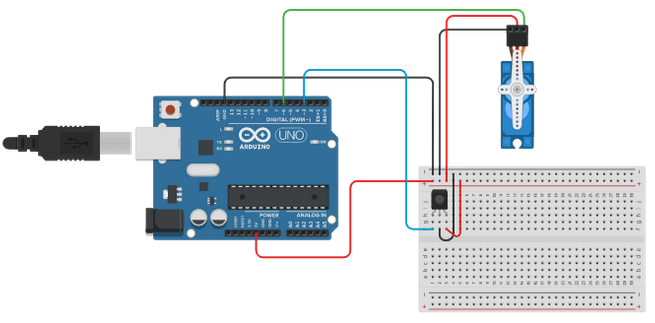
\includegraphics[scale=0.5]{Imagens/Experimentos/11-ServoMotor/esq.png}
	\caption{Esquemático do circuito do experimento 11.}
	\label{figExp11esq}
\end{figure}

\section{Sensor de Temperatura}
O objetivo desse experimento é utilizar um sensor para realizar a leitura da temperatura do ambiente e mostrar o valor em um display de 7 segmentos de 4 dígitos.

A pinagem do sensor de temperatura pode ser visto na Figura \ref{figDHT11}.

\begin{figure}[H]
	\centering
	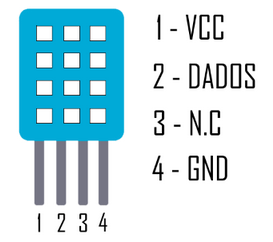
\includegraphics[scale=0.5]{Imagens/Experimentos/12-SensorTemperatura/dht11.png}
	\caption{Pinagem do sensor DHT11.}
	\label{figDHT11}
\end{figure}

O pino 1 do sensor deve ser ligado em 5V. O pino GND deve ser ligado ao GND do Arduino. O pino 2 deve ser ligado a porta analógica A0.

A Figura \ref{fig7seg4dig} mostra a pinagem do display de 7 segmentos com 4 dígitos.

\begin{figure}[H]
	\centering
	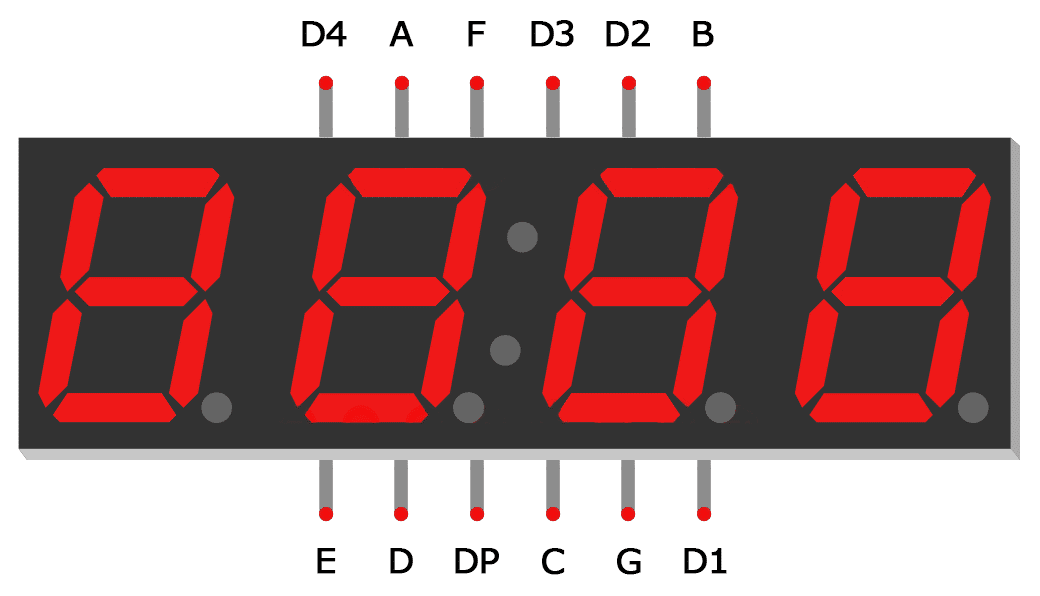
\includegraphics[scale=0.15]{Imagens/Experimentos/12-SensorTemperatura/7seg.png}
	\caption{Pinagem do display de 7 segmentos com 4 dígitos.}
	\label{fig7seg4dig}
\end{figure}

Como o \textit{Tinkercad} não possui os componentes utilizados para esse experimento, a simulação desse experimento não está disponível no site.

A Tabela \ref{tabSensorTemp} mostra as conexões que devem ser feitas entre o display e o Arduino.

\begin{table}[H]
	\centering
	\begin{tabular}{|c|c|}
	\hline
	\textbf{Display} & \textbf{Arduino} \\ \hline
	A                & 2                \\ \hline
	B                & 3                \\ \hline
	C                & 4                \\ \hline
	D                & 5                \\ \hline
	E                & 6                \\ \hline
	F                & 7                \\ \hline
	G                & 8                \\ \hline
	DP               & 9                \\ \hline
	D1               & 10               \\ \hline
	D2               & 11               \\ \hline
	D3               & 12               \\ \hline
	D4               & 13               \\ \hline
	\end{tabular}
	\caption{Conexões entre o Arduino e o display.}
	\label{tabSensorTemp}
\end{table}

\bibliographystyle{sbc}
\bibliography{referencias}

\end{document}
